\documentclass{article}

% if you need to pass options to natbib, use, e.g.:
% \PassOptionsToPackage{numbers, compress}{natbib}
% before loading nips_2018

% to compile a preprint version, e.g., for submission to arXiv, add
% add the [preprint] option:
% \usepackage[preprint]{nips_2018}

% to compile a camera-ready version, add the [final] option, e.g.:
% \usepackage[final]{nips_2018}

% to avoid loading the natbib package, add option nonatbib:
% \usepackage[nonatbib]{nips_2018}

\usepackage[utf8]{inputenc} % allow utf-8 input
\usepackage[T1]{fontenc}    % use 8-bit T1 fonts
\usepackage[hidelinks]{hyperref}       % hyperlinks
\usepackage{url}            % simple URL typesetting
\usepackage{booktabs}       % professional-quality tables
\usepackage{amsfonts}       % blackboard math symbols
\usepackage{nicefrac}       % compact symbols for 1/2, etc.
\usepackage{microtype}      % microtypography
\usepackage{adjustbox}
\usepackage{tikz}

\usepackage{pgfplots}
\usepgfplotslibrary{groupplots}
% \pgfplotsset{compat=1.13}


\usepackage{amsmath}
\usepackage{amssymb}
\usepackage{xfrac}
\usepackage{subfigure} 
\usepackage{floatrow}

\newcommand{\etal}{\textit{et al}.}
\newcommand{\ie}{\text it{i}.\textit{e}.}
\newcommand{\eg}{\textit{e}.\textit{g}.}

\newcommand{\MW}[1]{{\color{blue} {\bf (MW: #1)}}}
\newcommand{\AY}[1]{{\color{purple} {\bf (AY: #1)}}}
\newcommand{\SM}[1]{{\color{green} {\bf (SM: #1)}}}

\newcommand{\newl}{\newline}
\newcommand{\bm}{\mathbf}

\newcommand{\bW}{\bm{W}}
\newcommand{\bV}{\bm{V}}
\newcommand{\bD}{\bm{D}}
\newcommand{\bx}{\bm{x}}
\newcommand{\bh}{\bm{h}}
\newcommand{\bz}{\bm{z}}
\newcommand{\bb}{\bm{b}}




\newcommand{\mbC}{\mathbb{C}}
\newcommand{\mbR}{\mathbb{R}}


\title{Gated Complex Recurrent Neural Networks}

% The \author macro works with any number of authors. There are two
% commands used to separate the names and addresses of multiple
% authors: \And and \AND.
%
% Using \And between authors leaves it to LaTeX to determine where to
% break the lines. Using \AND forces a line break at that point. So,
% if LaTeX puts 3 of 4 authors names on the first line, and the last
% on the second line, try using \AND instead of \And before the third
% author name.

\author{
  Moritz Wolter and Anglea Yao \\%\thanks{Use footnote for providing further
    % information about author (webpage, alternative
    % address)---\emph{not} for acknowledging funding agencies.} \\
  Institute of Computer Science\\
  Bonn University\\
  \texttt{wolter@cs.uni-bonn.de} \\
  %% examples of more authors
  %% \And
  %% Coauthor \\
  %% Affiliation \\
  %% Address \\
  %% \texttt{email} \\
  %% \AND
  %% Coauthor \\
  %% Affiliation \\
  %% Address \\
  %% \texttt{email} \\
  %% \And
  %% Coauthor \\
  %% Affiliation \\
  %% Address \\
  %% \texttt{email} \\
  %% \And
  %% Coauthor \\
  %% Affiliation \\
  %% Address \\
  %% \texttt{email} \\
}

\begin{document}
% \nipsfinalcopy is no longer used

\maketitle

\begin{abstract}
Complex numbers have long been favoured for digital signal processing, yet complex representations rarely appear in deep learning architectures.  RNNs, widely used to process time series and sequence information, could greatly benefit from complex representations.  We present a novel complex gate recurrent cell.  When used together with norm-preserving state transition matrices, our complex gated RNN exhibits excellent stability and convergence properties.  We demonstrate competitive performance of our complex gated RNN on the synthetic memory and adding task, as well as on the real-world task of human motion prediction.
% In short we optimize: 
% \begin{align}
% \min_{\mathbf{W}} \text{cost}(\{\mathbf{x}\}, \{\mathbf{W}\}) \\
% \text{such that } \forall m \; \| \phi_m \| = 1, \\
%                   \forall n \; \| f'(h_n) \| \leq 1.
% \end{align}
% Where $\{\mathbf{W}\}$ denotes the set of network weights $\{\mathbf{x}\}$ the set of network inputs and $\{\phi_m\}$ the set of all weight matrix eigenvalues and finally $\|f'(h_n) \|$ the hidden actication derivatives.
% We show that our complex gated memory cells are practically stable and use wirtinger calculus to overcome limitations on skalar activations set by Liouville's theorem. It turns out that we do not need to work with a constrained optimization algorithm here, but can instead rewrite the problem in an unconstrained way, and use libraries optimized for large scale unconstrained optimization such as tensorflow or pytorch.
\end{abstract}

% ~\AY{overall storyline: we are interested in RNNs that are easy to optimize (stable for learning) and also able to learn long-term relationships -- this can be done via (1) gating and (2) norm-preserving matrices and (3) working in the complex domain, which we combine together.
% our insight is that 
% - in both real and complex, un-normalized GRUs, require bounded non-linearities e.g. tanh/Hirose; (to prove this first point, we need 2 plots, one for real, one for complex, each plot has 4 curves - bounded vs. unbounded, normalized vs. unnormalized) --> start with complex plot, if time we can add real; similar effects of the norm preservation has been observed with batch normalization as an alternative (real GRU with ReLU, find citation)
% - ReLU is able to solve the memory problem, whereas the Hirose/tanh is not; this we prove by showing in the bounded case, the Hirose is still not able to solve the memory problem well, vs. the ReLU, \ie it is really the choice in the non-linearity and not the unitary state transition matrices which solves the memory problem (we can show with the basic uRNN).


% "ortho-normalize" a matrix 
% }


\section{Introduction}
Recurrent neural networks (RNNs) are widely used for processing time series and sequential information.  The difficulties of training RNNs, especially when trying to learn long-term dependencies, are well-established, as RNNs are prone to vanishing and exploding gradients~\cite{bengio1994learning,Hochreiter,Pascanu}.  Heuristics developed to alleviate some of the optimization instabilities and learning difficulties include gradient clipping~\cite{goodfellow, Mikolov}, gating~\cite{cho-al-emnlp14,Hochreiter}, and using norm-preserving state transition matrices~\cite{Arjovsky, Hyland, Jing, Wisdom}.

Gating, as used in gated recurrent units (GRUs)~\cite{cho-al-emnlp14} and long short-term memory (LSTM) networks~\cite{Hochreiter}, have become common-place in recurrent architectures.  Gates facilitate the learning of longer term temporal relationships~\cite{Hochreiter}.  Furthermore, in the presence of noise in the input signal, gates can protect the cell state from undesired updates, thereby improving overall stability and convergence.

A matrix $\bm{W}$ is norm-preserving if its repeated multiplication with a vector leaves the vector norm unchanged, \ie $\Vert \bm{W} h\Vert_{2} = \Vert h \Vert_2$. 
Norm-presrving state transition matrices are particularly interesting for RNNs because they preserve gradients over time~\cite{Arjovsky}, thereby preventing both the vanishing and exploding gradient problem. To be norm-preserving, state transition matrices need to be either orthogonal or unitary\footnote{Unitary matrices are the complex analogue of orthogonal matrices, \ie~a complex matrix $W$ is unitary if $W \overline{W} = \overline{W} W = I$, where $\overline{W}$ is its conjugate transpose and $I$ is the identity matrix.}. Working with unitary matrices, in the complex domain, can be advantageous since unitary matrices are a larger and more expressive set than orthogonal matrices. Unitary matrices can spread their eigenvalues over the entire unit circle, whereas orthogonal matrices can only have eigenvalues of $\pm1$.  % Secondly, it is easier to develop computationally efficient parameterizations of unitary matrices as opposed to orthogonal ones~\cite{Arjovsky,Hyland,Jing}.\MW{Are we certain this is True? Working with Givens rotations or Housefolder reflections on the Reals can be implemented in an extreamly efficient way.}

%Rather than focusing on orthogonal matrices, however, Arjovsky~\etal~\cite{Arjovsky} and works in a similar vein~\cite{Jing, Hyland, Wisdom} advocate learning networks in the complex domain for two reasons.

%and more computationally efficient to enforce unitarity than orthogonality~\cite{Arjovsky}\AY{is this true? citations?}\MW{I think this is false, the math in the wisdom paper is pretty much identical for both cases.}.  
Complex numbers have long been favoured for signal processing~\cite{hirose2013complex,Li,Mandic}.  A complex signal does not simply double the dimensionality of the signal. Instead, the representational richness of complex signals is rooted in its physical relevance and the mathematical theory of complex analysis. Complex arithmetic, and in particular multiplication, is different from its real counterpart and allows us to construct novel network architectures with several desirable properties. Despite networks being complex-valued, however, it is often necessary to work with real-valued cost functions and or existing real-valued network components. Mappings from $\mathbb{C} \to \mathbb{R}$ are therefore indispensable.  Unfortunately such functions violate the Cauchy-Riemann equations and are not complex- differentiable in the traditional sense.  We advocate the use of Wirtinger calculus~\cite{Wirtinger} (also known as CR-calculus~\cite{Delgado}), which makes it possible to define complex (partial) derivatives, even when working with non-holomorph or non-analytic functions. 

Complex-valued representations have begun receiving some attention in the the deep learning community but they have been applied only to the most basic of architectures~\cite{Arjovsky,Guberman,Trabelsi}. For recurrent networks, complex representations could gain more acceptance if they were shown to be compatible with more commonly used gated architectures and also competitive for real-world data. This is exactly our aim in this current work, where we propose a complex-valued gated recurrent network and show how it can easily be implemented with a standard deep learning library (TensorFlow) that offers limited support for complex calculus. Our contributions can be summarized as follows.
\begin{itemize}
    \item We introduce a novel complex-gated recurrent unit; to the best of our knowledge, we are the first to explore such a structure using complex number representations.  
    \item We compare experimentally the effects of a bounded versus unbounded non-linearity in recurrent networks, finding evidence countering the commonly held heuristic that only bounded non-linearities should be applied in RNNs.  Unbounded non-linearities, in our case, perform better, but must be coupled with the stabilizing measure of using norm-preserving state transition matrices.
    \item Our complex gated network is stable and fast to train; it outperforms state-of-the-art with equal parameters on both synthetic tasks and the real-world application of predicting poses in human motion capture.   
\end{itemize}

% We also explore several non-linear activation and gating functions and make performance-based recommendations according to experiments on both synthetic and real-world tasks.     

% \AY{conclusion here is that the unbounded non-linearity, modReLU is better than the bounded Hirose on memory problem, comparable on the adding problem, however, modReLU must be used in conjunction with weight matrix normalization, or normalized in some other way, e.g. batch normalization in the real case, for complex, we investigat other possibilites in the future. }

\section{Related work}
The current body of literature in deep learning focuses predominantly on real-valued neural networks. Theory for learning with complex-valued data, however, was established long before the breakthroughs of deep learning. % ~\cite{Brandwood,Franken,van1994complex}. %Applications to neural network cost functions where considered later \cite{Mandic}. All solutions essentially utilize Wirtinger calculus \cite{Wirtinger}, to come up with an approximate gradient for a non-holomorph function. 
This includes the development of complex non-linearities and activation  functions~\cite{georgiou1992complex,kim2001complex,uncini1999complex}, the computation of complex gradients and Hessians~\cite{van1994complex,zimmermanncomparison}, and complex backpropagation~\cite{benvenuto1992complex,Brandwood,Franken,goh2004complex,kim2002fully,leung1991complex}. 

Complex-valued representations were first used in deep networks to model phase dependencies for more biologically plausible neurons~\cite{reichert2013neuronal} and to augment the memory of LSTMs~\cite{danihelka2016associative}. Recently, complex-valued CNNs have been proposed as an alternative for classifying natural images~\cite{Guberman,Trabelsi} and inverse mapping of MRI signals~\cite{Virtue}.  Complex CNNs were found to be competitive or better than state-of-the-art~\cite{Trabelsi} and significantly less prone to over-fitting~\cite{Guberman}. %Using the Cauchy-Riemann equations~\cite{Trabelsi} conclude that many currently used complex activations are non-holomorph and proceed by defining their own framework for dealing with non-holomorph functions which are real differentiable, without referencing the existing work in \cite{Brandwood}\cite{Bos}\cite{Franken}\cite{Delgado}\cite{Mandic}. We argue that Wirtinger calculus should be used as a tool to theoretically understand the properties of the pseudo-gradients used to backpropagate trough non-holomorph functions.

For working with temporal sequences, complex-valued RNNs have also been explored~\cite{Arjovsky,Hyland,jing2016tunable,Wisdom}, though interest in complex representations stems from improved learning stability. In~\cite{Arjovsky}, norm-preserving state transition matrices are used to prevent vanishing and exploding gradients.  Since it is difficult to parameterize real-valued orthogonal weights,~\cite{Arjovsky} recommends shifting to the complex domain, resulting in a unitary RNN (uRNN). The weights of the uRNN in~\cite{Arjovsky}, for computational efficiency, are constructed as a product of component unitary matrices.  As such, they span only a reduced subset of unitary matrices and do not have the expressiveness of the full set.  Alternative methods of parameterizing the unitary matrices have been explored~\cite{Hyland,jing2016tunable,Wisdom}. Our proposed complex gated RNN builds on these works in that we also use unitary state transition matrices.  In particular, we adopt the parameterization of~\cite{Wisdom} in which weights are parameterized by full-dimensional unitary matrices, though any of the other parameterizations~\cite{Arjovsky,Hyland,jing2016tunable} can also be substituted.

%Gating has been shown to be highly beneficial for temporal sequence modeling~\cite{cho-al-emnlp14,Hochreiter}. 
% The gated orthogonal RNN~\cite{Jing} is similar in spirit to our proposed network.  

% their state to state update equation is based on an efficient implementation of the restricted set of orthogonal rotations SO(3). Matrices in SO(3) have a determinant of one. Since the product of all eigenvalues is the determinant, their eigenvalues are fixed to be one.

% Using optimisation methods introduced by \cite{Tagare} and popularised for use with RNNs by \cite{Wisdom} we propose an unresctriced complex GRU, which can spread out its eigenvalues over the entire unit circle. \cite{Jing}, uses only real gates, which are identical to gates previously explored in the literature. We explore novel complex definitions. 

% A holomorph non-linearity was used in \cite{Guberman}, \cite{Arjovsky} introduces a novel non-linearity which is not complex-differentiable. \cite{Trabelsi} compares complex non-linearities and systematically measures performance. Furthermore complex batch-normalization is introduced.

\section{Preliminaries}
We represent a complex number $z \in \mbC$ as $z = x + ib$, where $x = \Re{(z)}$ and $y = \Im{(z)}$ are the real and imaginary parts respectively.  The complex conjugate of $z$ is $\bar{z} = x - iy$.  In polar coordinates, $z$ can be expressed as $z = |z| e^{i\theta_z}$, where $|z|$ and $\theta$ are the magnitude and phase respectively %, where $x = r \cos(\theta)$ and $y = r \sin(\theta)$.  We also use 
%where $r = |z|$ 
and $\theta_z=\text{atan2}(x,y)$. Note that $z_1\cdot z_2 = |z_1||z_2|e^{i(\theta_1 + \theta_2)}$, $z_1 + z_2 = x_1 + x_2 + i(y_1 + y_2)$ and $s\cdot z = s\cdot r e^{i\theta}, s \in \mathbb{R}$. The expression $s\cdot z$ scales $z$'s magnitude, while leaving the phase intact. 

\subsection{Complex Gradients}
A complex-valued function $f : \mbC \to \mbC$ can be expressed as $f(z) = u(x,y) + i v(x,y)$ where $u(\cdot,\cdot)$ and $v(\cdot,\cdot)$ are two real-valued functions.  The complex derivative of $f(z)$, or the $\mbC$-derivative, %is ``complex-differentiable'' in $z$ 
is defined if and only if $f$ is \emph{holomorph}. % in $z$.  
In such a case, the partial derivatives of $u$ and $v$ %with respect to $x$ and $y$ 
must not only exist but also satisfy the Cauchy-Riemann equations, where $\sfrac{\partial u}{\partial x} = \sfrac{\partial v}{\partial y}$ and $\sfrac{\partial v}{\partial x} = - \sfrac{\partial u}{\partial y}$.

Strict holomorphy can be overly stringent for deep learning purposes.  In fact, Liouville's theorem~\cite{Liouville} states that the only complex function which is both holomorph and bounded is a constant function. This implies that for complex (activation) functions, one must trade off either boundedness %, and accept the existence of singularities, 
or differentiability. One can forgo holomorphy and still leverage the theoretical framework of Wirtinger or CR-calculus~\cite{Delgado,Mandic} to work separately with the $\mbR$- and $\overline{\mbR}$- derivatives\footnote{For holomorph functions the $\overline{\mbR}$-derivative is zero and the $\mathbb{C}$- derivative is equal to the $\mbR$-derivative.} %\SM{$\Re(x)$ or $\mbR$ ?}: %; these are partial derivatives with respect to $z$ and $\bar{z}$ and are defined as
\begin{equation}
    \mbR\text{-derivative} \triangleq \frac{\partial f}{\partial z}|_{\bar{z}=\text{const}}\mkern-18mu = \frac{1}{2}(\frac{\partial f}{\partial x} - i \frac{\partial f}{\partial y}),\; \overline{\mbR}\text{-derivative} \triangleq \frac{\partial f}{\partial \bar{z}}|_{z=\text{const}}\mkern-18mu = \frac{1}{2}(\frac{\partial f}{\partial x} + i \frac{\partial f}{\partial y}).
\end{equation}
Based on these derivatives, one can define the chain rule for a function $g(f(z))$ as follows:
\begin{equation}
    \frac{\partial g(f(z))}{\partial z} = \frac{\partial g}{\partial f} \frac{\partial f}{\partial z} + \frac{\partial g}{\partial \bar{f}} \frac{\partial \bar{f}}{\partial z} \qquad \text{where} \qquad \bar{f} = u(x,y) - iv(x,y).
\end{equation}
Since mappings from $\mathbb{C} \to \mathbb{R}$ can generally be expressed in terms of the complex variable $z$ and its conjugate $\bar{z}$, the Wirtinger-Caclulus allows us to formulate and theoretically understand the gradient of real-valued loss functions in an easy yet principled way.

\subsection{A Split Complex Approach}

We work with a split-complex approach, where we apply real-valued non-linear activations to process the real and imaginary parts of the complex number separately. This makes it convenient for implementation purposes, since standard deep learning libraries are not designed to work with complex representations natively. Instead, we can simply keep track of complex numbers as two separate real-valued components. Split complex activation functions process either the magnitude and phase, or the real and imaginary components separately with two real-valued nonlinear functions and then recombine the two into a new complex quantity,  % $f(z) = f_r(x) + if_r(y)$. This approach allows us to work with bounded real activations such as the sigmoidal function or the hyperbolic tangent. While boundedness is one advantage, which may result from the split complex approach, the these non-linearities are not fully complex functions, which consitently modifiy magnitude and phase. Fully complex functions $f(z) = f_c(z)$ such as hyperbolic tangents, the complex exponential or moebius transforms are holomorph, have proper gradients, but are not bounded and come with singularities.

While some may argue this takes away from the utility of having complex representations, we prefer this to fully complex functions. Fully complex non-linearities do exist and may seem favourable (as argued by~\cite{Trabelsi}, one would then only need to keep track of two derivatives) but due to Liouville's theorem, we must forgo boundedness and then deal with forward pass instablities.  

% ~\AY{explain what split complex approach is, motivate why we want to ork with a split complex approach:
% \begin{itemize}
% \item because we are already using C-R calculus, which conveniently partitions the partials wrt to the real / imaginary parts
% \item implementation-wise, is convenient since current machine learnign packages do not offer support for complex numbers and derivatives, so int he implementation one needs to track the real and imaginary parts separately anyhow, as real-valued numbers wrt to x and y
% \item conveniently allows us to work with bounded non-linearities
% \end{itemize}

\section{Complex Gated RNNs}

\subsection{Basic Complex RNN Formulation}

Without any assumptions on real versus complex representations, we define a basic RNN as follows: 
\begin{align}
    \bz_{t} &= \bW \bh_{t-1} + \bV \bx_{t} + \bb \label{eq:basicRNN1}\\
    \bh_{t} &= f_a(\bz_{t}) \label{eq:basicRNN2}
\end{align}

where $\bx_t$ and $\bh_t$ represent the input and hidden unit vectors at time $t$.  $f_a$ is a point-wise non-linear activation function, and $W$ and $V$ are the hidden and input state transition matrices respectively.  In working with complex networks, $\bx_t \in \mathbb{C}^{n_h \times 1}$, $\bh_t \in \mathbb{C}^{n_h \times 1}$, $\bW \in \mathbb{C}^{n_h \times n_h}$ and $\bV \in \mathbb{C}^{n_h \times n_{in}}$, where $n_x$ and $n_h$ are the dimensionalities of the input and hidden states respectively.

\subsection{Complex Non-linear Activation Functions}~\label{sec:nonlinearity}
\begin{figure}
    \centering
    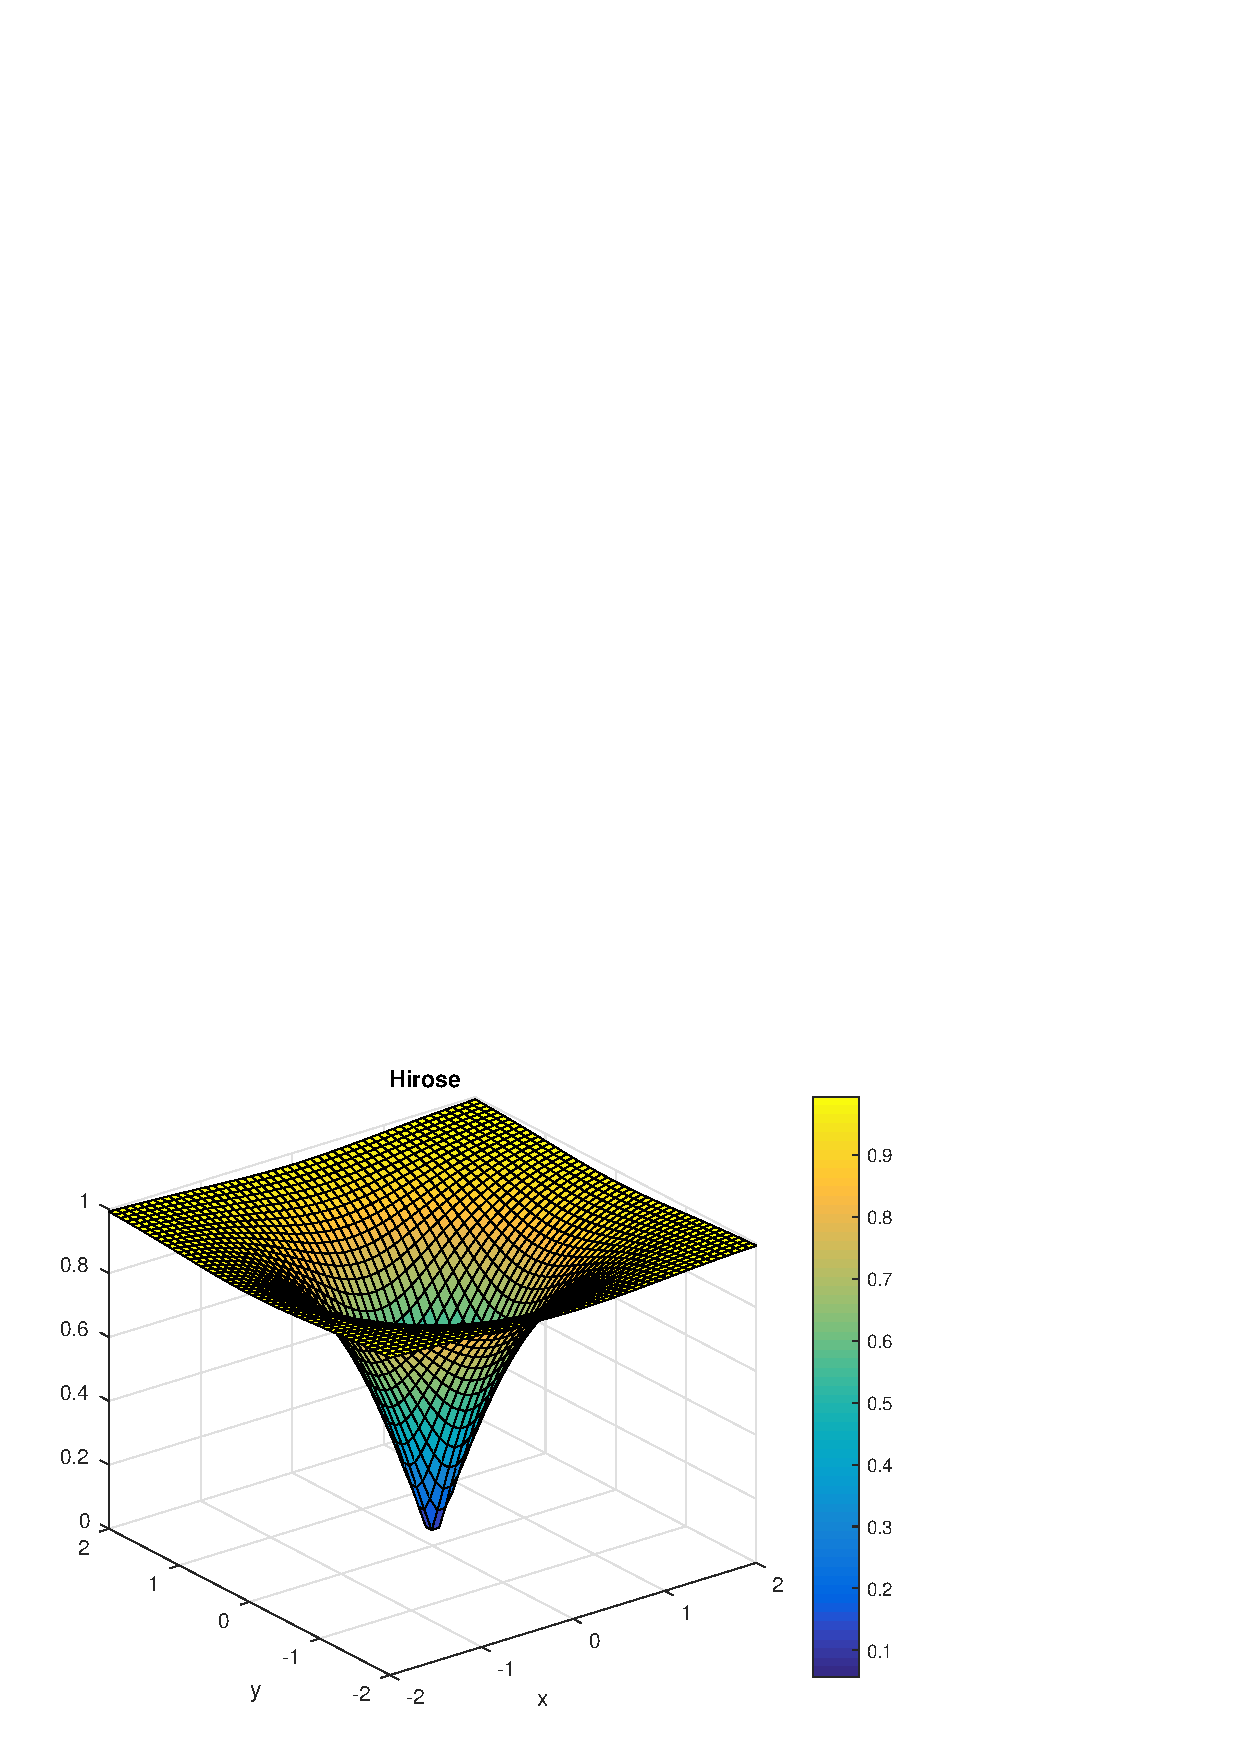
\includegraphics[width=0.45\linewidth]{./img/Hirose_slice.pdf}
    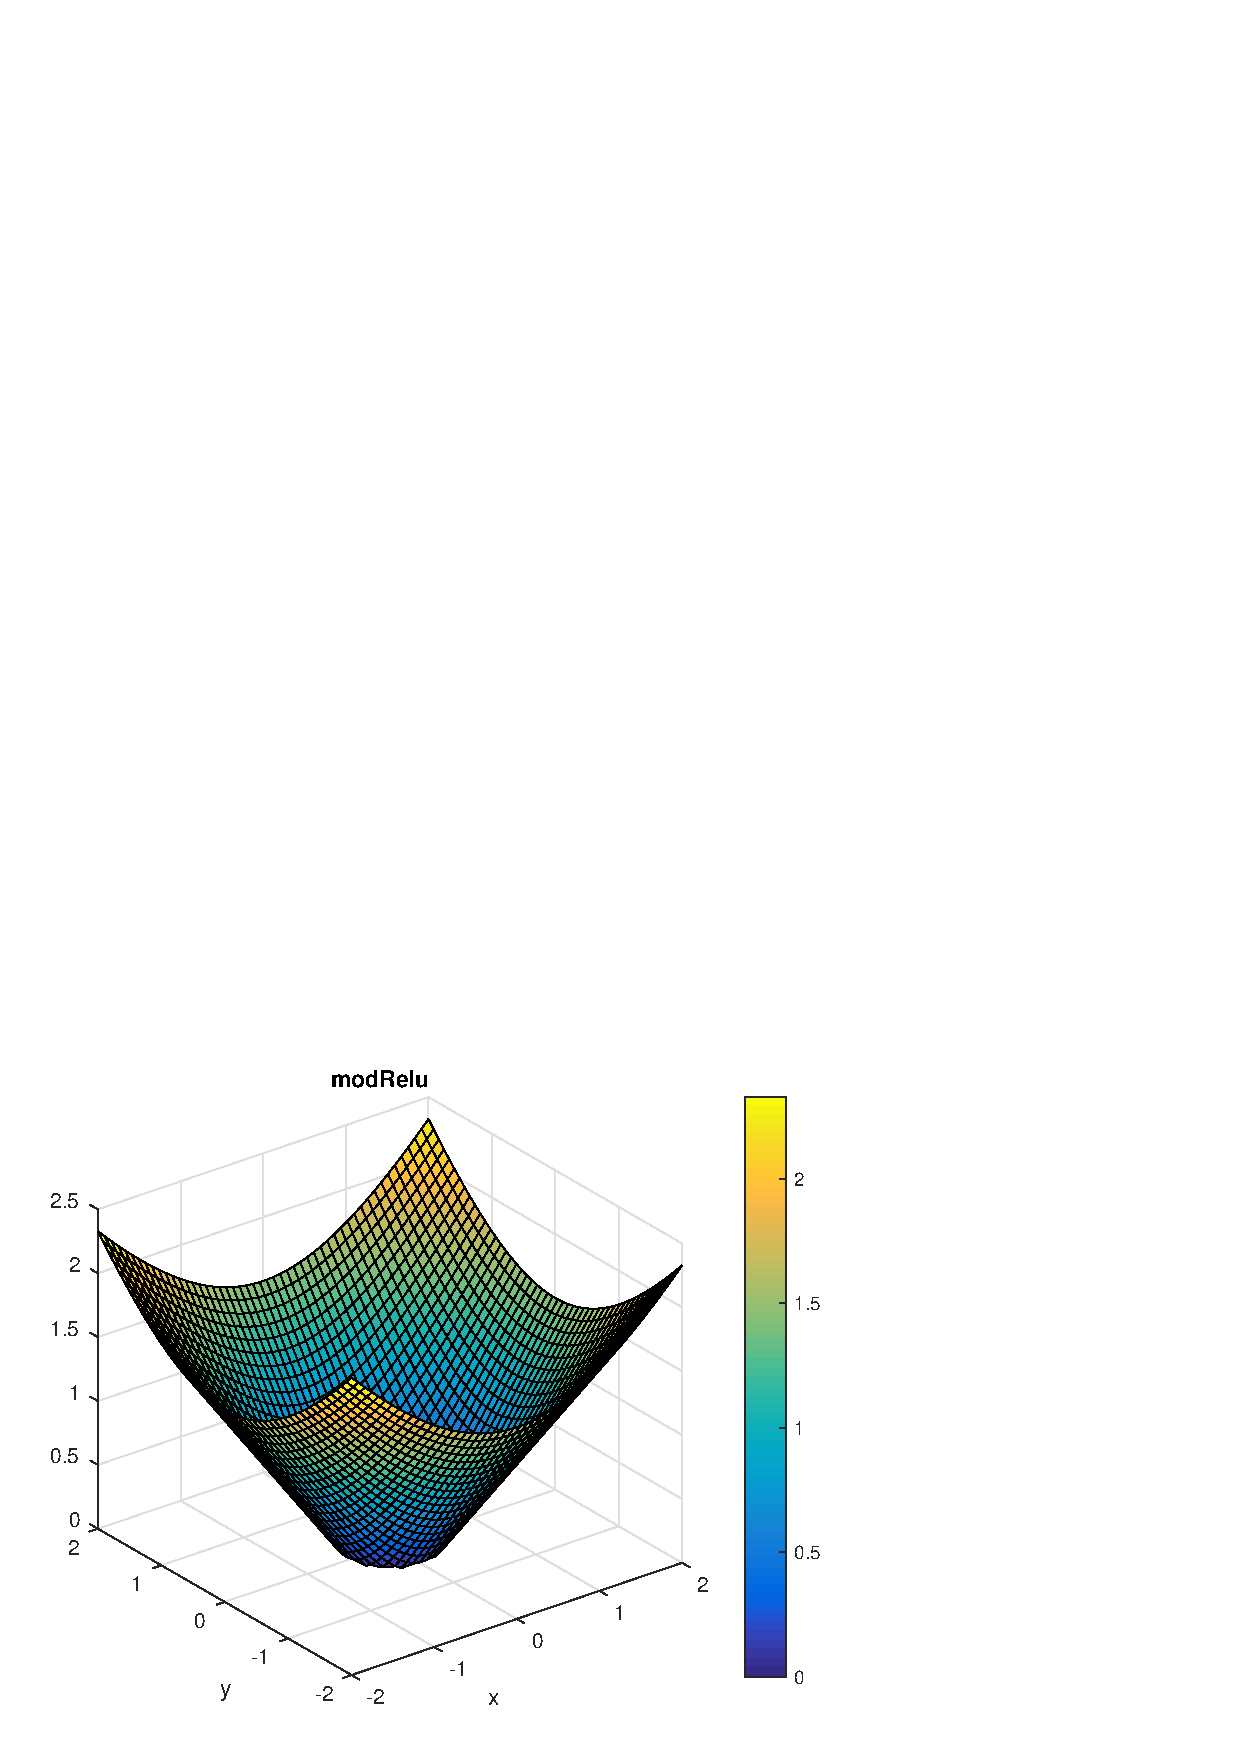
\includegraphics[width=0.45\linewidth]{./img/modRelu_slice.pdf}
    \caption{Surface plots of the magnitude of the Hirose and modRelu activation functions, the modRelu uses b=-0.5.}
    \label{fig:hiroseModRelu}
\end{figure}

Choosing a non-linear activation function $f_a$ for complex networks can be non-trivial.  Liouville's theorem~\cite{Liouville} stipulates the necessity of trading off boundedness for differentiability.  Though holomorph non-linearities using transcendental functions have also been explored in the literature~\cite{Mandic}, the presence of singularities makes them difficult to learn in a stable manner.  Instead, bounded non-holomorph non-linearities tend to be favoured~\cite{hirose2013complex,Mandic}, where bounded real-valued non-linearities are applied to the split complex.  This also parallels the convention of using (bounded) $\tanh$ non-linearities in real RNNs.
%A split complex activation functions process the real and imaginary separately using two real-valued nonlinear functions and recombine the two into complex quantity $f(z) = f_r(x) + if_r(y)$. This approach allows us to work with bounded real activations such as the sigmoidal function or the hyperbolic tangent. While boundedness is one advantage, which may result from the split complex approach, the these non-linearities are not fully complex functions, which consitently modifiy magnitude and phase. Fully complex functions $f(z) = f_c(z)$ such as hyperbolic tangents, the complex exponential or moebius transforms are holomorph, have proper gradients, but are not bounded and come with singularities.

A common split is with respect to the magnitude and phase.  This non-linearity was popularized by Hirose~\cite{hirose2013complex} and scales the magnitude by a factor $m^2$ before passing it through a $\tanh$: 
\begin{equation}~\label{eq:Hirose}
    f_{\text{Hirose}}(z) = \tanh\left(\frac{|z|}{m^2}\right)e^{-i \cdot \theta_z} = \tanh\left(\frac{|z|}{m^2}\right)\frac{z}{|z|}.
\end{equation}

In other areas of deep learning, the rectified linear unit (ReLU) is now the go-to choice as a non-linearity.  In comparison to sigmoid / $\tanh$ activations, they are computationally cheap, and have been shown to not only expedite convergence~\cite{Krizhevsky} but also perform better~\cite{Nair,Maas,Zeiler}.  However, there is no direct extension into the complex domain, and as such, modified versions have been proposed~\cite{Guberman,Virtue}, with the most popular being the modReLU~\cite{Arjovsky}.  The modReLU is a variation of the Hirose non-linearity, where the $\tanh$ on the magnitude is replaced with a ReLU:
\begin{equation}~\label{eq:modrelu}
    f_{\text{modReLU}}(z) = \text{ReLU}(|z| + b)e^{-i \cdot \theta_z} = \text{ReLU}(|z| + b)\frac{z}{|z|},
\end{equation}

and $b$ denotes an offset parameter.  % By switching out the $\tanh$ with a ReLU, the modReLU inverts the active region of the Hirose non-linearity.  

\subsection{$\mbR \to \mbC$ input and $\mbC \to \mbR$ output mappings}
While several time series problems are inherently complex, especially when considering their Fourier representations, the majority of benchmark problems in machine learning are still only defined in the real number domain. However, one can still solve these problems with complex representations, since a real $z$ has simply a zero imaginary component, \ie $\Im{(z)} = 0$ and $z = x + i\cdot 0$.

%However transformations from the real number onto the complex domain such as the Fourier or Hilbert transform could be used as mappings from $C$ to $R$.
To map the complex state $\bm{h}$ into a real output $\bm{o}_r$, we use a linear combination of the real and imaginary components, similar to~\cite{Arjovsky}, with $\bm{W}_o$ and $\bm{b}_o$ as weights and offset:
\begin{equation}
 \bm{o}_r = \mathbf{W}_o [\Re(\mathbf{h}) \; \Im(\mathbf{h})] + \mathbf{b}_o.
\end{equation}

\subsection{Optimization on the Stiefel Manifold for Norm Preservation}~\label{sec:stability}

In~\cite{Arjovsky}, it was proven that a unitary~\footnote{Since $\mbR \subseteq \mbC$, we use the term unitary to refer to both real orthogonal and complex unitary matrices and make a distinction for clarity purposes only where necessary.} $\bW$ would prevent vanishing and exploding gradients of the cost function $C$ with respect to $h_t$, since the gradient magnitude is bounded.  However, this proof hinged on the critical assumption that the derivative of $f_a$ is also unity.  This assumption is valid if the pre-activations are real and one chooses the ReLU as the non-linearity.  For complex pre-activations, however, this is no longer a valid assumption. Neither the Hirose non-linearity (Eq.~\ref{eq:Hirose}) nor the modReLU (Eq.~\ref{eq:modrelu}) can guarantee stability (despite the suggestion otherwise in the original proof~\cite{Arjovsky}). % , see detailed derivation in Supplementary materials). %As such, gradients in the uRNN, when used together with the modReLU, do not remain constant as is otherwise suggested in the proof by~\cite{Arjovsky}.  

Even though it is not possible to guarantee stability, we strongly advocate using norm-preserving state transition matrices, since they do still have excellent stabilizing effects.  This was proven experimentally in~\cite{Arjovsky,Hyland,Wisdom} and we find similar evidence in our own experiments (see Fig.~\ref{fig:unnGRU}).  Ensuring that $\bm{W}$ remains unitary during the optimization can be challenging, especially since the group of unitary matrices is not closed under addition.  As such, it is not possible to learn $\bW$ with standard  update-based gradient descent.  Alternatively, one can learn $\bW$ on the Stiefel manifold~\cite{Wisdom}, with the $k+1$ update $\bW_{k+1}$ given by~\cite{Tagare}
% Stiefel manifold described in\cite{Tagare}. Tagare proposes to use a gradient, which points along the Stiefel-Manifold of unitary matrices, which
% itself unitary. This gradient may be computed using \cite{Tagare}:
\begin{align}
\mathbf{W}_{k+1} &=  (\mathbf{I} + \frac{\lambda}{2}\mathbf{A}_k)^{-1}(\mathbf{I} - \frac{\lambda}{2}\mathbf{A}_k)\mathbf{W}_k \qquad \text{where} % \qquad \mathbf{A} &= \mathbf{W}\frac{\partial F}{\partial \mathbf{W}}^* - \mathbf{W}^*\frac{\partial F}{\partial \mathbf{W}}
\qquad \mathbf{A} &= \mathbf{W}\nabla_{\overline{\bm{w}}}{F} - \overline{\mathbf{W}}\nabla_{{\bm{w}}}{F}
\label{eq:Stiefel}
\end{align}
and where $\lambda$ is the learning rate, $\bm{I}$ the identity matrix, and $F$ the cost function.%, and $\bm{W}^*$ the conjugate transpose.%,  $\nabla F$ the %numerical gradient values 
% gradient of the cost function $F$ with respect to variable $\mathbf{W}$ and $^*$ denotes the conjugate transpose.


%, % $\bz \in \mathbb{C}$,
 % however, neither Hirose non-linearity nor the modReLU full the amplitude the the modReLU as proposed by Arjovsky~\etal~\cite{Arjovsky} and 

\subsection{Complex-Valued Gating Units}
In keeping with the spirit that gates determine the amount of a signal to pass, we construct a complex gate as a $\mathbb{C}^{n_h \times n_h} \to \mathbb{R}^{n_h \times 1}$ mapping.  Like in real gated RNNs, the gate is applied as an element-wise product, \ie $\bm{g} \odot \bh = \bm{g} \odot |\bm{h}| e^{i\theta_h}$.  In our complex case, this type of operation results in an element-wise scaling of the hidden state's magnitude. When the gate is 0, it completely reset a signal, whereas if it is 1, then it ensures that the signal is passed entirely.     %This creates a novel type of gating which ensures that parts of the Thereby creating a novel memory type, which has parts of its memory shielded from gate interference.
We introduce our gates into the RNN in a similar fashion as the classic GRU~\cite{cho-al-emnlp14}:
\begin{align}
    \widetilde{\bz}_{t} &= \bW (\bm{g}_r \odot \bh_{t-1}) + \bV \bx_{t} + \bb \label{eq:state_candidate} \\
    \bh_{t} &= \bm{g}_z \odot f_a(\widetilde{\bz}_t) +(1 - \bm{g}_z) \odot \bh_{t-1}, \label{eq:state_update}
\end{align}
where $\bm{g}_r$ and $\bm{g}_z$ represent reset and update gates respectively and are defined with corresponding subscripts $r$ and $z$ as
\begin{align}
    \bm{g}_r = f_g(\bz_r), \qquad \text{where} \qquad \bz_r = \bW_r \bh + \bV_r \bx_t + \bb_r, \label{eq:dual_gate1} \\
    \bm{g}_z = f_g(\bz_z), \qquad \text{where} \qquad \bz_z = \bW_z \bh + \bV_z \bx_t + \bb_z.
    \label{eq:dual_gate2}
\end{align}

Above, $f_g$ denotes the gate activation, $\bW_r \in \mathbb{C}^{n_h \times n_h}$ and $\bW_z \in \mathbb{C}^{n_h \times n_h}$ denote state to state transition matrices, $\bV_r \in \mathbb{C}^{n_h \times n_i}$ and $\bV_z \in \mathbb{C}^{n_h \times n_i}$ the input to state transition matrices, and $\bm{b}_r \in \mathbb{C}^{n_h}$ and $\bm{b}_z \in \mathbb{C}^{n_h}$ the biases.  $f_g$ is a non-linear gate activation function. We choose for $f_g$ a sigmoid product: %There are several options for $f_g$, including a sigmoid product:

\begin{equation}
    f_{\text{ prod}}(\bz) = \sigma(\Re{(\bz)}) \cdot \sigma (\Im{(\bz)}).
    \label{eq:prod_sigma}
\end{equation}

This formulation is active in the first quadrant, where both real and imaginary part are positive.

As mentioned previously, even with unitary state transition matrices, this type of gating is not mathematically guaranteed to be stable.  However, the effects of vanishing gradients are mitigated by the fact that the derivatives are distributed over a sum~\cite{Hochreiter,cho-al-emnlp14}. Exploding gradients are clipped.


% Other alternatives include a sum formulation:
% ~\AY{isn't the sigma taking inside, not outside of the two values?}
% \begin{equation}
%     f_{\text{ sum}}(\bz)_ = \sigma(a \Re{(\bz)}) + b \Im{(\bz)})
%     \label{eq:sum_sigma}
% \end{equation}
% with $a, b \in \mathbb{R}$ and $0 < a < 1$ and $0 < b < 1$ this gate activation creates a sigmoid-like hill, with learnable steepness and orientation. 
% \begin{equation}
%     f_{\text{ Hirose}}(\bz) = \tanh\left(\frac{|\bz|}{m}\right) \cdot \sigma(a\theta_z + b).
%     \label{eq:gate_hirose}
% \end{equation}
% \MW{I think these two gate activations should go, since we did not manage to show a significant benefit of using these.}
% Finally the last gate activation takes inspiration from Hirose to take magnitude information into account while explicitly gating on the phase. Parameter $a$ controls the steepness of the sigmoid, which is necessary because unlike in $\mathbb{R}$, where the input is not bounded, the phase $\theta_z$ is the output of an atan2-function and therefore $\theta \in [-\pi, \pi]$. $b$ allows us to initialise the gate in an open manner. For $m \in \mathbb{R}$ we require $m > 0$, to prevent the gate from producing negative outputs.
% A major difference with respect to real valued memory cells. This definition allows the model to scale data points according to their current relevance, while leaving phase information untouched. \\

% \subsection{A Stable Complex Gate}
% ~\AY{the double gate version is not stable, we introduce a new way of coupling the gates}

% % To limit the number of additional parameters introduced by the gating mechanism we also explore using the real and imaginary parts of the gating equation $\mathbf{g}$, to do the gating.

% \begin{align}
% \bz_c & = \bW_c \bh + \bV_c \bx_t + \bb_c \label{eq:complex_coupled}\\
% \bm{g}_{r} & = \text{ReLU} (\Re(\mathbf{z_c})), \quad
% \bm{g}_{z} = \text{ReLU} (\Im(\mathbf{z_c})).
% \end{align}

% We use a single gate equation containing the weights $\bW_c \in \mathbb{C}^{n_h \times n_h}$, $\bV_c \in \mathbb{C}^{n_h \times n_i}$ and $\bb_c \in \mathbb{C}^{n_h}$.  While this is less expressive than the GRU-styled , this definition reduces the number of parameters, but does not allow us to leverage the full expressiveness of the complex domain.
% \MW{TODO: Reduction, add the numbers}
% % ~\MW{Add $\sigma_{mod} = \tanh(r/m)\sigma(a\theta)$ if reults turn out to be ok.}
% % We interpret the contents of the gate vectors as a measure of their corresponding state entries current relevance, with one indicating the value is important and should be kept, while zero indicates it should be deleted. 
% % The modRelu fits nicely into this arcitecture, because it allows us to learn a threshold $b$. State entries which have been scaled by the gates to be smaller than $b$ should be forgotten. 

% Given that complex values are more representation, we can also couple the gates to a common pre-activation, the same pre-activation. 
% This version is interesting because we theoretically understand the conditions required for stability (see appendix). However using unitary or split orthogonal  
% gate "stability" - doesn't really matter since we need (1) saturation behaviour and (2) non-linearity makes the whole setup unstable anyway
% \MW{TODO: add coupled gates based on ~\ref{eq:sum_sigma}.}


% In this section we introduce state dependency by taking the classic GRU~\cite{cho-al-emnlp14} to the complex domain,

\section{Experimentation}
\subsection{Synthetic Tasks: Memory and Adding Problem}

We test our complex gated RNN on two benchmark synthetic tasks: the memory problem and the adding problem~\cite{Hochreiter}.  These problems are designed especially to challenge RNNs, and require the networks to store information over time scales on the order of hundreds of time steps.  

In the \textbf{Memory Problem}, the RNN should remember $n$ inputs symbols over a time period of length $T + 2n$ based on a dictionary set $\{s^1, s^2, ..., s^n, s^b, s^d\}$, where $s^1$ to $s^n$ are symbols to memorize and $s^b$ and $s^i$ are blank and delimiter symbols respectively. The input sequence, of length $T + 2n$, is composed of $n$ symbols drawn randomly with replacement from $\{s^1, ..., s^n\}$, followed by $T-1$ repetitions of $s^b$, $s^d$, and another $n$ repetitions of $s^b$. The objective of the RNN, after being presented with the initial $n$ symbols, is to generate an output sequence of length $T + S$, with $T$ repetitions of $s^b$, and upon seeing $s^d$, recall the original $n$ input symbols.  A network without memory would output $s^b$ and once presented with $s^d$, randomly predict any of the original $n$ symbols; this results in a categorical cross entropy of $\sfrac{(n+1\log(8))}{(T+2(n+2))}$.% \SM{I put the braces around. }. 

In the \textbf{Adding Problem}, two sequences of length $T$ are given as input, where the first sequence consists of numbers randomly sampled from $\mathcal{U}[0,1]$\footnote{Note that this is a variant of~\cite{Hochreiter}'s original adding problem, which draws numbers from $\mathcal{U}[-1,1]$ and used three indicators  $\{-1,0,1\}$. Our variant is consistent with state-of-the-art~\cite{Arjovsky, Hyland, Wisdom}}, while the second is an indicator sequence of all $0's$ and exactly two $1's$, with the first $1$ placed randomly in the first half of the sequence and the second $1$ randomly in the second half.  The objective of the RNN is to predict the sum of the two entries of the first input sequence once the second 1 is presented in the indicator input sequence.  A naive baseline would predict $1$ at every time step, regardless of the input indicator sequence's value; this produces an mean squared error (MSE) of 0.167, \ie the variance of the sum of two independent uniform distributions. 

In our experiments, we choose $n=8$ and $T=250$ for the memory problem and $T=250$ for the adding problem. Previous works~\cite{Arjovsky, Hyland, Wisdom} have found that gating is not helpful for the memory problem, but can greatly help with the adding problem since it is able to ignore non-relevant inputs.

\subsection{Real-World Task: Human Motion Prediction}
We also apply our complex gated RNN to the real-world task of human motion prediction, \ie~predicting likely future $3D$ poses of a person given the past motion.  This task is of interest to diverse areas of research, including 3D tracking in computer vision~\cite{sigal2010humaneva,yao2012coupled}, motion synthesis for graphics~\cite{kovar2002motion,safonova2007construction} as well as pose and action predictions for assistive robotics~\cite{koppula2016anticipating}.  We follow the same experimental setting as~\cite{martinez2017human}, working specifically with the walking sequences of the Human 3.6M dataset~\cite{h36m_pami}.  For training, we use six of the seven actors and test on actor five.  We use the pre-processed data of~\cite{NIPS2006_3078}, which converts the motion capture into exponential map representations of each joint.  Based on an input sequence of body poses from 50 frames, the future 25 frames are predicted, with error measured by the difference in Euler angles with respect to the ground truth poses.

\subsection{RNN Implementation Details}
We work in Tensorflow, using RMS-prop to update standard weights and the multiplicative Stiefel-manifold update as described  Eq.~\ref{eq:Stiefel} for all unitary state transition matrices.  The unitary state transition matrices are initialized the same as~\cite{Arjovsky} as the product of component unitary matrices. % (for details, see Supplementary Materials).
All other weights are initialized using the uniform initialisation method recommended in~\cite{glorot2010understanding}, \ie  $U[-l,l]$ with $l=\sqrt{6 / (n_{in} + n_{out})}$, where $n_{in}$ and $n_{out}$ are the input and output dimensions of the tensor to be initialised.  All biases are intialized as zero, with the exception of the gate biases $\bm{b}_r$ and $\bm{b}_z$, which are initialized at 4 to ensure fully open gates and linear behaviour at the start of training.  All synthetic tasks are run for $2\cdot 10^4$ iterations with a batch-size of 50 and a constant learning rate of 0.001 for both the RMS-Prop and the Stiefel-Manifold updates.

For the human motion prediction task, we use the same learning rate as~\cite{martinez2017human}, $0.005$, though we reduce our state size to 512 (to be compatible with their 1024\footnote{Note that this is a larger reduction than necessary -- the approximately equal state size is $\sqrt{\frac{1024^2}{2}}$}). 

\subsection{Results}

\subsubsection{Impact of Gating}
We first look at the impact that gating has on the synthetic tasks by comparing our complex gated RNN with the gateless uRNN from~\cite{Arjovsky} (see Fig.~\ref{fig:unnGRU}). Both networks use complex representations and also unitary state transition matrices. As additional baselines, we also compare with TensorFlow's out-of-the-box GRU and LSTM.  We choose the hidden state size $n_h$ of each network to ensure that the resulting number of parameters is approximately equivalent ($\sim 165000$)\footnote{The total number of LSTM weights depends on the output dimension, which is nine in the case of the memory problem and one for the adding problem, we adapted the LSTM state size to $n_h=800$ for the adding problem to keep the total number of parameters at approximately 165k.}.

\begin{figure}[t!]%
\centering
\subfigure[]{%
\includegraphics[width=0.4\linewidth]{./img/aaai_GRU_UNN_cgRNN_memory.pdf}}
\qquad
\subfigure[]{%
\includegraphics[width=0.4\linewidth]{./img/aaai_GRU_UNN_cgRNN_adding.pdf}}%
    \caption{\small Comparison of our complex gated RNN (cgRNN, blue, $n_h\!=\!80$) with the unitary RNN~\cite{Arjovsky}(uRNN, orange, $n_h\!=\!140$) and standard GRU~\cite{cho-al-emnlp14}(orange, $n_h\!=\!112$) on the memory (a) and adding (b) problem for $T\!=\!250$. The hidden state size $n_h$ for each network are chosen so as to approximately match the number of parameters (approximately 42k parameters total).  Figure best viewed in colour.  On the memory problem, having norm-preserving state transition matrices is critical for stable learning, while on the adding problem, having gates is important.}
    \label{fig:unnGRU}
    \vspace{-0.5cm}
\end{figure}

We find that our complex gated RNN successfully solves both the memory problem as well as the adding problem.  On the memory problem, gating does not play a role. Instead, having norm-preserving weight matrices is key to ensure stability during the learning.  Without it, both the GRU and the LSTM are highly unstable and while the GRU is eventually able to solve the problem, it takes many more iterations.  The LSTM fails to solve the problem and stays at the baseline.  Our gated complex RNN achieves very similar performance as the uRNN.  This has to do with the fact that we initialize our gate bias term to be fully open, \ie $\mathbf{g}_r = \mathbf{1}$, $\mathbf{g}_z = \mathbf{1}$.  Under this setting, the formulation is the same as the uRNN, and the $\bm{W}$ will dominate the cell's dynamics.  

For the adding problem, previous works~\cite{Arjovsky,Hyland,Wisdom} have suggested that gates are beneficial.  We confirm this result and speculate that the advantage comes from the gates shielding the network from the irrelevant inputs of the adding problem, hence the success of our complex gated RNN as well as the GRU and LSTM, but not the uRNN.  We are very surprised to discover that the standard GRU baseline, without any norm-preserving state transition matrices works very well on the adding problem; in fact marginally outperforms our complex gated RNN.  However, we believe this result does not speak to the inferiority of complex representations, rather that the adding problem as a synthetic task is not able to leverage the advantages offered by the representation.  

\subsubsection{Non-Linearity Choice and Norm Preservation}

\begin{figure}[t!]
    \centering
\subfigure[]{%
\includegraphics[width=0.4\linewidth]{./img/aaai_stiefel_bounded_memory.pdf}}
\qquad
\subfigure[]{%
\includegraphics[width=0.4\linewidth]{./img/aaai_stiefel_bounded_adding.pdf}}%
    \caption{\small Comparison of non-linearities and norm preserving state transition matrices on the complex gated RNNs for the memory (a) and adding (b) problems for T=250.  We find that the unbounded modReLU (see Eq.~\ref{eq:modrelu}) performs best for both problems, but only if the state transition matrices are kept unitary.  Without unitary state-transition matrices, the bounded Hirose non-linearity (see Eq.~\ref{eq:Hirose}) performs better. We use $n_h=80$ for all experiments.}
    \label{fig:complex_results}
    \vspace{-0.5cm}
\end{figure}

We compare the bounded Hirose $\tanh$ non-linearity versus the unbounded modReLU (see Section~\ref{sec:nonlinearity}) in our complex gated RNN in Figure~\ref{fig:complex_results} and discover a strong interaction effect from the norm-preservation.  First, we find that optimizing on the Stiefel manifold to preserve norms for the state transition matrices significantly improves learning, regardless of the non-linearity.  In both the memory and the adding problem, keeping the state transition matrices unitary ensures faster and smoother convergence of the learning curve. 

Without unitary state transition matrices, the bounded $\tanh$ non-linearity, \ie the conventional choice is better than the unbounded modReLU.  However, with unitary state transition matrices, the modReLU pulls ahead.  Again, this result is consistent for both the memory and the adding problem.  We speculate that the modReLU, like the ReLU in the real setting, is a better choice of non-linearity.  The advantages afforded upon it by being unbounded, however, also makes it more sensitive to stability, which is why these advantages are present only when the state-transition matrices are kept unitary.  Similar effects were observed in real RNNs in~\cite{Ravanelli2017ImprovingSR}, in which batch normalization was required in order to learn a standard RNN with the ReLU non-linearity.

\subsubsection{Choosing a gate activation}
TODO...


\subsubsection{Human Motion Prediction}
\begin{figure}[b]
    \centering
    \subfigure[]{\adjustbox{raise=5pc}{\scalebox{.9}{
        \begin{tabular}{|c|c|c|}\hline
            seed     &   cgRNN-error                    & GRU-error                      \\ \hline
            0080     &   \textbf{1.13}                  & 1.24                           \\
            0160     &   \textbf{1.14}                  & 1.30                           \\
            0320     &   \textbf{1.19}                  & 1.31                           \\
            0400     &   \textbf{1.17}                  & 1.34                           \\
            0560     &   \textbf{1.23}                  & 1.39                           \\
            1000     &   \textbf{1.39}                  & 1.51                           \\ \hline
            average  &   \textbf{1.21}                  & 1.35                           \\ \hline
        %\bottomrule
    \end{tabular}
    }}}
    \subfigure[]{%
    \includegraphics[width=0.4\linewidth]{./img/euler.pdf}
    }
    \caption{\small Motion prediction Euler angle errors for the complex gated RNN (green) versus GRU (blue), where each line indicates a separate test sequence.  The final error after $20,000$ iterations is shown in the adjacent table.}
    \label{fig:euler}
\end{figure}

Figure~\ref{fig:euler} shows the test-set Euler-errors of six different walking sequences during training. As suggested by~\cite{martinez2017human} a test run is done every 1000 iterations. Our complex gated RNN consistently improves the prediction results in comparison to a GRU with more than twice the state size. All weights except for the unitary state transition matrices are updated using stochastic gradient descent.  The final Euler error for the sequences are shown in the table in Figure~\ref{fig:euler}; we observe that our complex gated RNN has about $10\%$ lower error than the standard GRU.  

\section{Conclusion}
In this paper, we have proposed a novel complex gated recurrent unit which we use together with unitary state transition matrices to form a stable and fast to train recurrent neural network.  To enforce unitarity, we optimize the state transition matrices on the Stiefel manifold, which we show to work well with the modReLU.  Our complex gated RNN achieves state-of-the-art performance on the adding problem while remaining competitive on the memory problem.  % In our experiments Showing that Stiefel-Manifold optimisation of unitary state matrices can be beneficial in aated architectures, we introduce complex gating. This is no trivial task. Various options have been explored. We recommend double gating with a product sigmoid gate activation.
We further demonstrate the applicability of our network on the real-world task of human motion prediction, in which we show superior performance with respect to a real-valued GRU.  In future work, we intend to apply Fourier and Hilbert transform pre-processing on the temporal data to fully leverage the complex representations.
\bibliographystyle{plain}
\bibliography{literature}
\end{document}